\chapter{Summative Evaluation}

I evaluated Sketch It, Make It in two ways. First, I tested SIMI
with 60 undergraduate architecture students. The objective was to test
if (and how well) SIMI's sketch-based interaction could be used to
make precisely-defined designs for fabrication. Second, a task-tool
analysis compares the strategy of an experienced SIMI user (me) for
making an object with that of an experienced Illustrator user. This
was done to compare how these starkly different tools require
designers to work.

\begin{figure}
  \centering
  \begin{subfigure}[t]{0.6\textwidth}
    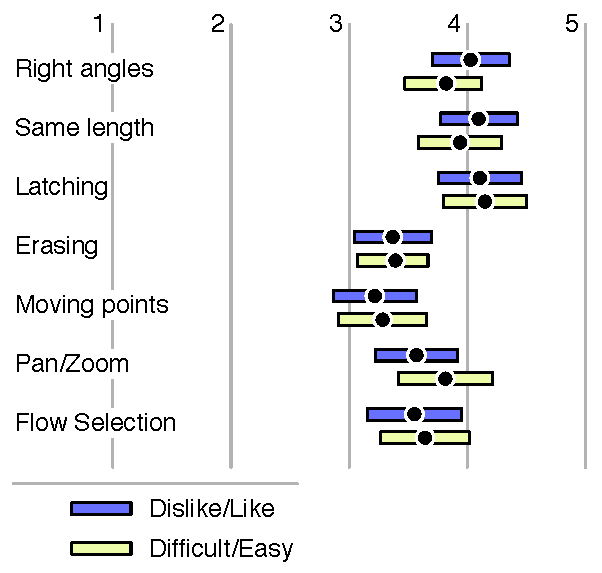
\includegraphics[width=\linewidth]{img/feature-attitude-and-ease.pdf}
    \caption{Questions about features: attitude and ease of use.}
    \label{fig:survey-feature-ease-attitude}
  \end{subfigure}
  \\
  \vspace{5mm}
  \begin{subfigure}[t]{0.8\textwidth}
    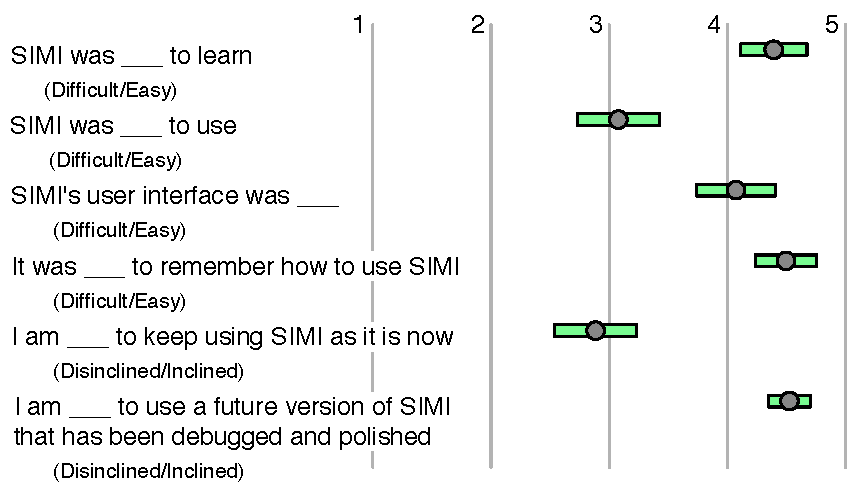
\includegraphics[width=\linewidth]{img/program-attitude-2.pdf}
    \caption{Questions on the system as a whole.}
    \label{fig:survey-program-attitude}
  \end{subfigure}
  \caption[Workshop Survey Results]{Survey results from the workshop
    with undergraduate architecture students. 40 students responded to
    the questionnaire.}
  \label{fig:survey}
\end{figure}


\section{Workshop}

I held a workshop with 60 undergraduate architecture students to
gather qualitative feedback about how easy or difficult SIMI is to
learn and use. The workshop was held in 30-minute sessions over two
days in a room equipped with iMacs and Wacom Intuos
tablets. Regrettably, these tablets do not display output, so users'
eyes are not focused on the same physical location as the pen
tip---leading to significant hand-eye coordination challenges. More
costly display tablets like the Cintiq (Figure~\ref{fig:simi-intro})
avoid this problem, but were unavailable for the workshop.

Initially, students complained that the tablet hardware was difficult
to use, but most of the tablet-related trouble went away after about
ten minutes. Then they quickly learned to make line work and
constraints. At first they had trouble erasing and selecting points,
but soon learned to make these gestures.

I expected students to have difficulty using SIMI because the hardware
(tablets) and interaction paradigm (sketch-based modeling) were both
new to them. However, by the second day, most questions and comments
regarded missing features, not about how to use the system.

After the workshop, students were offered an extra credit assignment
to complete a short survey. This generated 40 responses, summarized in
Figure~\ref{fig:survey}. The survey had three sets of questions, all
on a 5-point scale. The first set asked how easy (or hard) each
interaction method was to use. The second set of questions measured
the student's attitude about the techniques. This line of questioning
was borrowed from~\cite{bae-everybody}.

Only the Erase and point selection gestures seemed to give
participants trouble. These are the only gestures that depend on
timing. Erasing must be done with a quick, vigorous shake of the
pen. Selecting points must be done quickly, or SIMI will interpret the
input as the beginning of a flow selection.

The last set of questions polled students about their perception of
the program as a whole: e.g. how easy it was to learn, to use, and
remember. Although the students reported the system was easy to
\textit{learn}, their responses indicate they found it difficult to
\textit{use}. This might be explained by the limited time available
(one hour), and the novelty of the hardware.

Finally, we asked (1) how much people would like to continue using the
system as it is currently, and (2) how likely they would be to try it
again when it was debugged and nicely tuned. The responses are in
stark contrast: most would not continue using SIMI as it is today,
owing to bugs and lack of features. Despite this, the response to the
second question was very positive.

Enthusiasm about the interaction paradigm of sketching was evident in
comments by respondents. For example:

\begin{itemize}
\item ``This is the start of a great program, and once it is polished it
  will be extremely useful.''
\item ``The program seems like it could be really cool to use in the
  future. I really enjoyed using a tablet and stylus. It made
  designing fun.''
\end{itemize}

Not all commentary was positive. Aside from complaints about bugs,
most negative comments concerned missing features (for example, a
constraint to make lines parallel).

\section{Task-Tool Analysis}

A second method to evaluate our system is to compare the actions
required to make an object with SIMI compared with those of a
conventional tool such as Illustrator.

An expert Adobe Illustrator user was asked to describe the sequence of
discrete actions necessary to model the table shown in
Figure~\ref{fig:table}. This designer has used Illustrator to make
dozens of laser-cut items.

\begin{samepage}
For example, the first three actions were:

\begin{enumerate}
\item Press the M key to enter rectangle drawing mode.
\item Type rectangle dimensions.
\item Place the rectangle on the drawing canvas.
\end{enumerate}
\end{samepage}

The first action is a persistent mode change, while the second two
specify values. A similar transcript was recorded for SIMI. Five
categories were used to code the verbal protocol. They are listed in
Table~\ref{tab:task-tool-protocol}.


\begin{table}%[h] % [h]ere [t]op [b]ottom [p]age
\centering
\begin{tabular}{l | p{11cm}}
\textbf{Action Type} & \textbf{Description} \\
\hline
&\\

Persistent mode change & 

Change the tool input state so subsequent input is interpreted in
context of that tool (e.g. line drawing mode). User must enter another
persistent mode to exit the first.

\\

Specify value &

Specify a dimension or location.

\\

Specify target &

Indicate (select) an element for a subsequent operation.

\\

Transformation &

Apply an operation that changes existing model elements beyond simply
specifying numeric values. Transformations include moving or erase
items.

\\

Transient mode change &

Temporarily change the tool mode so input is interpreted
differently. This kind of mode change is part of a phrase, and will
revert to another mode when the phrase is complete.

\\
\hline
\end{tabular}
\caption[Task-Tool Protocol Analysis Categories]{Action types used in the task-tool protocol analysis.}
\label{tab:task-tool-protocol}
\end{table}


\begin{figure}[h]
  \centering
  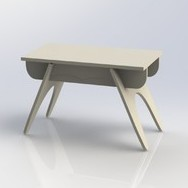
\includegraphics[width=0.4\linewidth]{img/table.jpg}
  \caption[Laser-cut Table Sold on Ponoko]{A laser-cut table for sale
    on Ponoko. We asked expert designers how they would replicate this
    object using either Illustrator or SIMI.}
  \label{fig:table}
\end{figure}

\begin{table}[h]
  \centering
  \begin{tabular}{ l c c }
    \textbf{Action type} & \textbf{Illustrator} & \textbf{SIMI} \\
    \hline
    Persistent mode change & 12 & 0 \\
    Specify value & 17 & 7 \\
    Specify target & 7 & 4 \\
    Transformation & 6 & 27 \\
    Transient mode change & 2 & 0 \\
    \hline
    & \textbf{44} & \textbf{38} \\
  \end{tabular}
  \caption[Action type frequency]{Frequency of action types in the
    design protocol of expert Adobe Illustrator and SIMI users. }
  \label{tab:expert}
\end{table}

The action frequency (listed in Table~\ref{tab:expert}) shows how the
two tools are used to create the same output. Roughly the same number
of actions was taken (Illustrator:~44, SIMI:~38).

To make an object using Illustrator, an expert issues a series of
\textit{Select, Specify} actions: either activate a persistent tool
(e.g. line mode) or select a modeling element (e.g. a line on the
screen), then specify a value or position by typing a number or moving
the mouse.

In contrast, most discrete actions with SIMI involve transforming
geometry that is already on the screen, for example, constraining two
existing lines to meet at a common point or form a right angle. A
single sketched gesture fluidly performs both \textit{Select} and
\textit{Specify} operations that require two distinct actions in
Illustrator. For example, right angle gesture necessarily indicates
the line segments to be constrained.

The Task-Tool Analysis discussed here is limited. Because there is
only one expert SIMI user (the author) it is not possible to gather
more than one protocol for that tool. However, if several users were
trained in SIMI, it would have been possible to collect more data.
The classification scheme summarized in
Table~\ref{tab:task-tool-protocol} not been vetted by researchers in
other contexts. Further, the protocols were rated by only one person,
leading to concerns with inter-rater reliability.

